\documentclass[11pt]{article}

\usepackage[letterpaper,margin=1in]{geometry}
\usepackage[T1]{fontenc}
\usepackage[utf8]{inputenc}
\usepackage{graphicx}
\usepackage[hidelinks]{hyperref}
\usepackage{enumitem}
\usepackage{booktabs}
\usepackage{tabularx}
\usepackage{wrapfig}

\graphicspath{{assets/}{report/assets/}}
\setlength{\parindent}{0pt}
\setlength{\parskip}{0.16em}
\setlist{noitemsep,topsep=1pt,leftmargin=1.15em}
\setlength{\emergencystretch}{1em}

\newcommand{\tightsection}[1]{\vspace{-0.25em}\section{#1}\vspace{-0.25em}}
\newcommand{\smallcaption}[1]{\vspace{-0.35em}{\footnotesize #1}\vspace{-0.3em}}

\title{\vspace{-2.2em}\textbf{Raw Power Matters. Team Fit Matters Too.}\\
\large ECS 163 Final Report}
\author{Team 13\\Yuhui Chen, Yuxiang Huang, Junhao Zhang, Jiayi Bai, Tingwei Zhang}
\date{}

\begin{document}
\maketitle
\vspace{-2.1em}

\tightsection{Motivations and Objectives}
Competitive Pokemon looks simple from the outside: a stronger Pokemon should have higher base stats, and higher stats should lead to more competitive use. Our project tests that intuition with a data story about VGC 2022. The central claim is that raw power matters, but team fit matters too. Competitive strength is partly individual and partly relational: usage is shaped by teammates, roles, moves, items, abilities, and repeated team structures.

The objective was to build a narrative visualization that can be understood by viewers who are not experts in competitive Pokemon. We did not want a broad Pokedex dashboard. Instead, the interface guides the viewer through one argument: base stat total alone is a weak explanation for competitive usage, while teammate connectivity and role evidence explain why Pokemon such as Incineroar remain highly valuable. The page uses a Martini Glass narrative structure \cite{segel2010narrative}: a guided opening, a contradiction, a network reveal, and finally open exploration.

\tightsection{Driving Application and Datasets}
The driving application is exploratory team analysis for the 2022 Video Game Championships (VGC) metagame. The user-facing question is: \textit{What really makes a Pokemon strong?} In the app, each Pokemon can be inspected as an individual statistical object and as a member of a team ecosystem.

We use two public datasets. The main source is the Complete Competitive Pokemon Database (May 2022), which includes Pokemon forms, base stats, monthly usage, VGC rule information, teammates, moves, items, and abilities \cite{carbone2022competitive}. The second source supplies Pokemon image assets for visual identity \cite{singh32000pokemon}. After preprocessing, the app loads 1,066 Pokemon/form rows, 2,606 teammate co-usage links, and 2,967 build records. The React app reads cleaned CSV files for Pokemon, team edges, build usage, and image lookup. It derives network degree, weighted teammate footprint, maximum teammate link, offensive and defensive scores, and usage/stat correlation summaries inside the front end.

\begin{figure}[h]
\centering
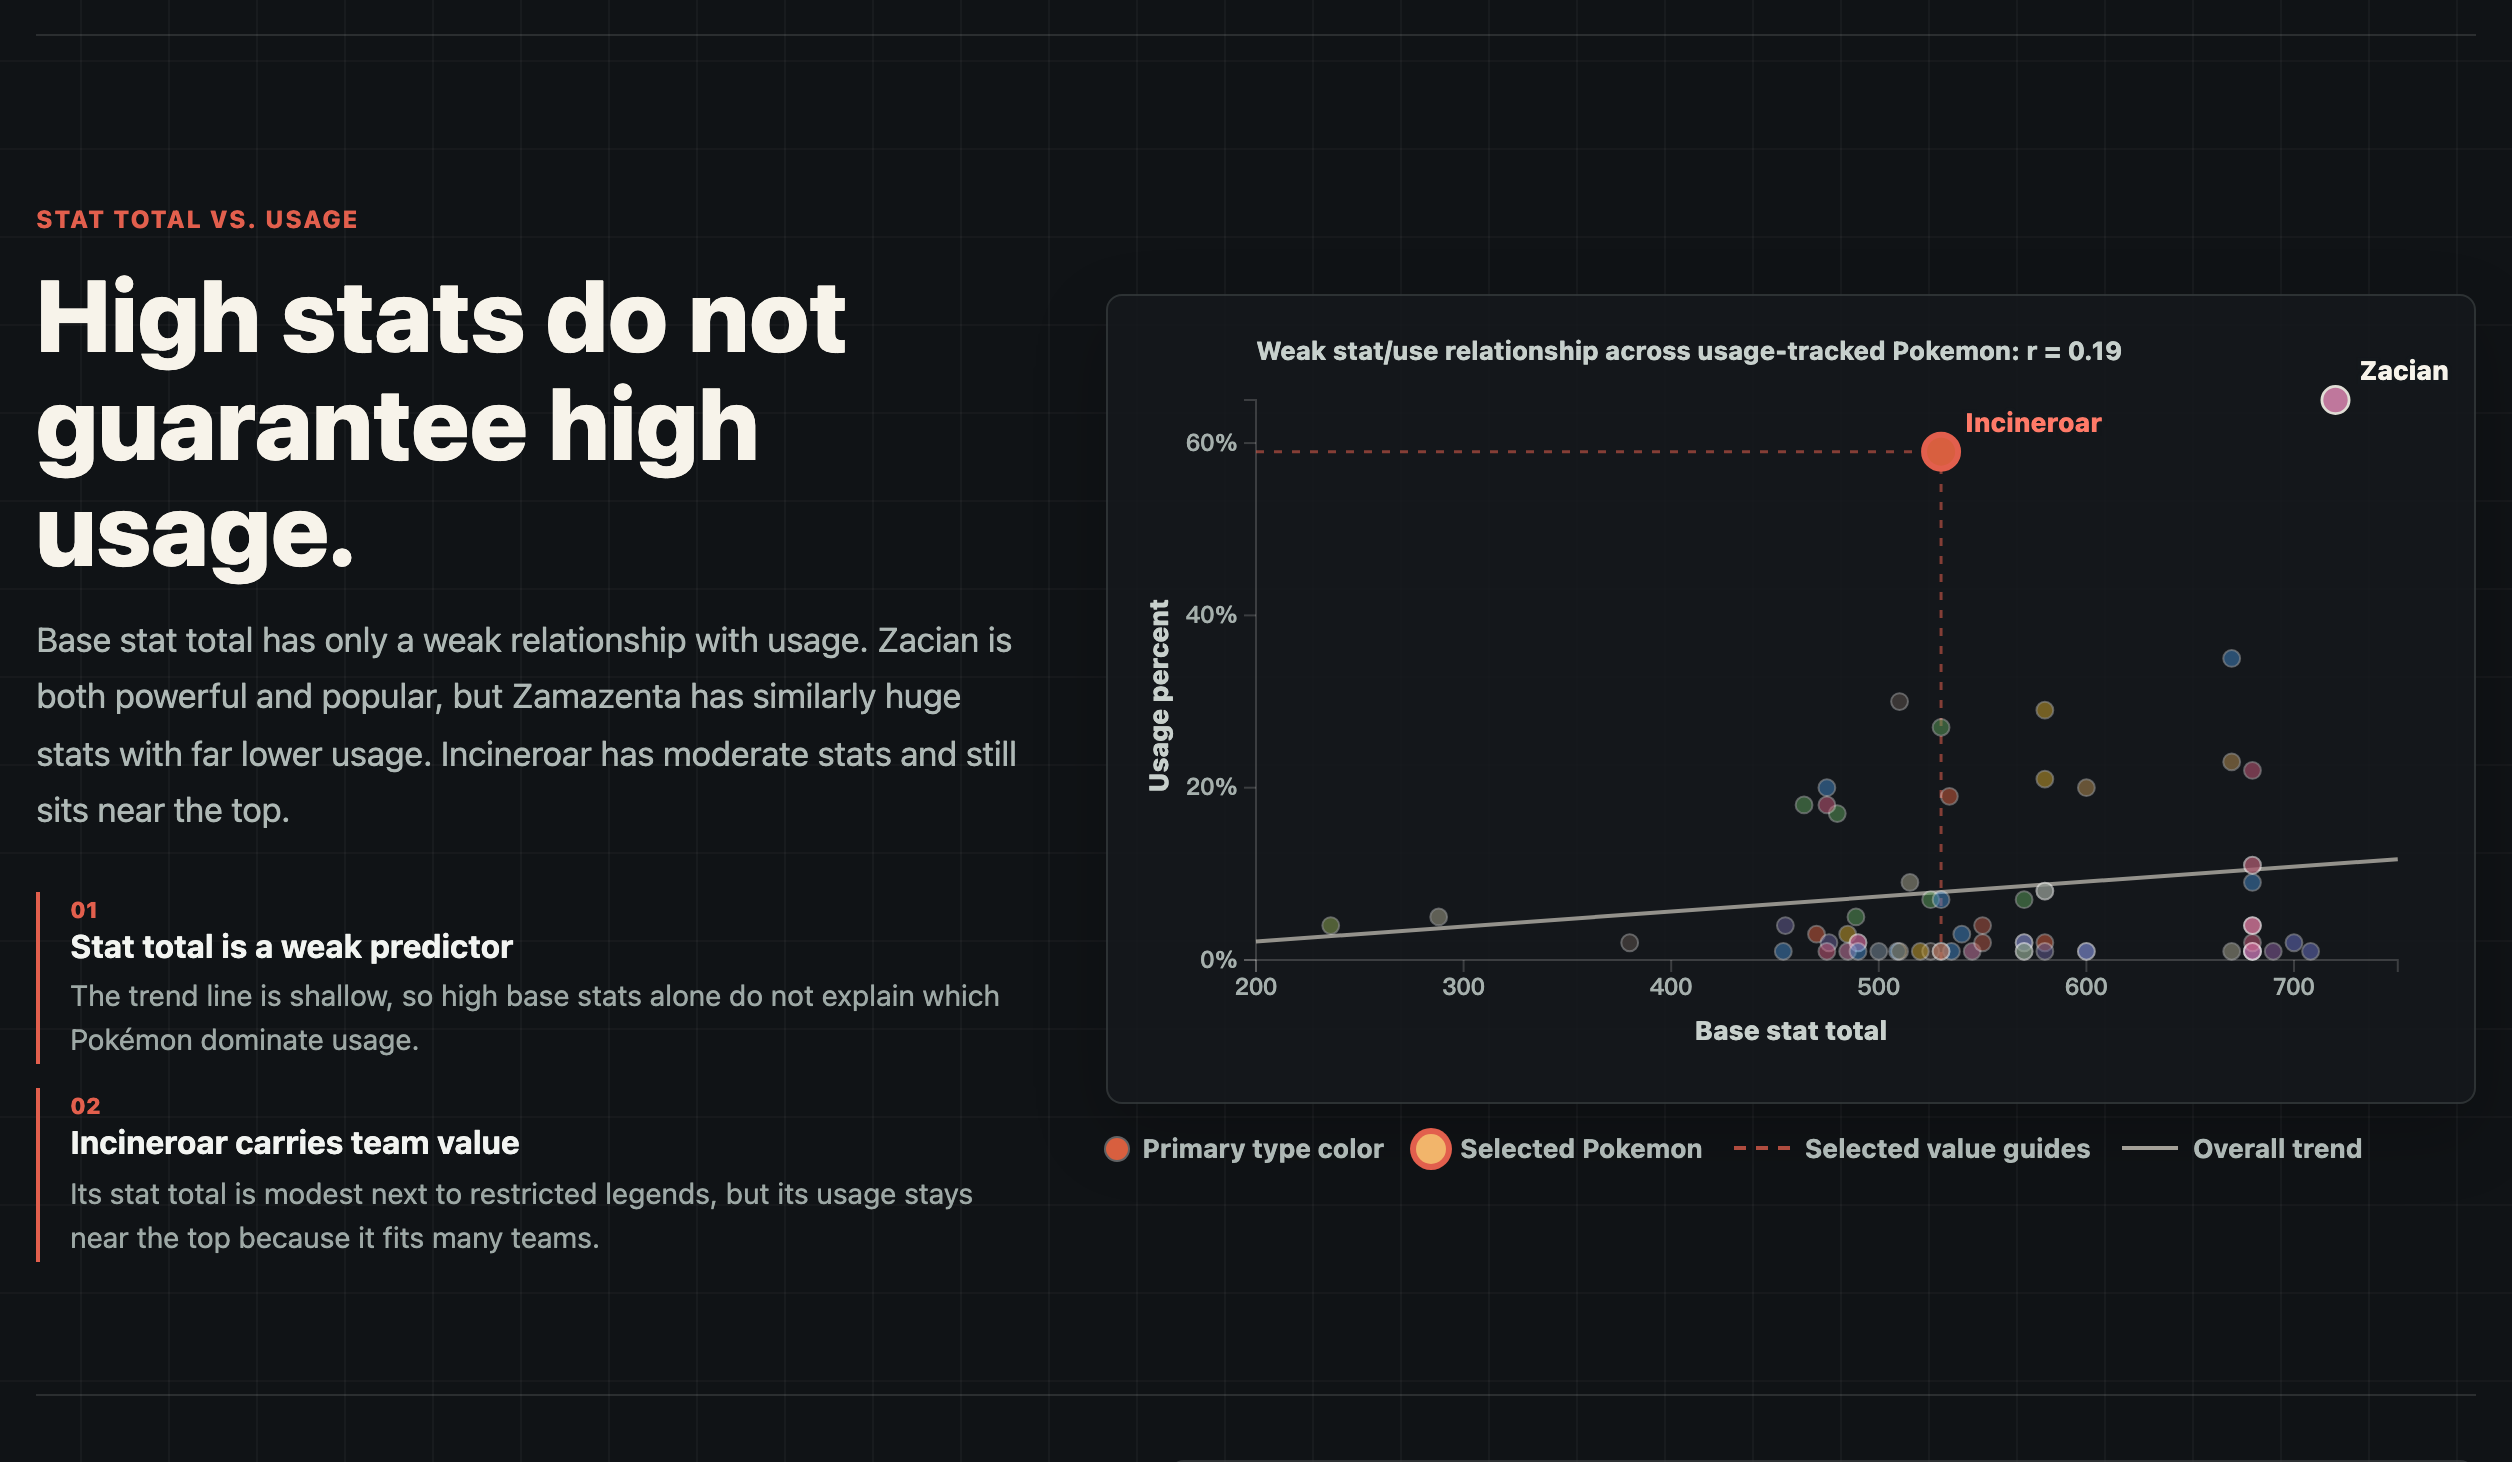
\includegraphics[width=0.88\linewidth]{figure_scatterplot_contradiction.png}
\smallcaption{Figure 1. The opening contradiction: base stat total has a weak relationship with competitive usage. Incineroar has moderate stats but high usage, while some high-stat Pokemon have low usage.}
\end{figure}

\tightsection{Challenges to Address}
The main challenge was restraint. The dataset contains enough information to make many separate charts, but too many views would dilute the story. We needed the visual design to make one argument clearly: competitive success cannot be read from raw stats alone. That meant cutting down the network to a readable subset, keeping the scatterplot focused on the contradiction, and turning moves/items/abilities into evidence instead of a long fact list.

Another challenge was network readability. Force-directed layouts can become visually noisy, especially with labels and images. We addressed this by limiting the graph to case-study Pokemon and high-signal team links, encoding usage with node size, using edge width for co-usage strength, and adding selection-based highlighting. Labels are reserved for story-relevant nodes and archetypes, while tooltips and the detail panel carry deeper information.

The third challenge was avoiding overclaiming. Usage is not the same as win rate, and co-usage edges do not prove causation. The design therefore frames connectivity as evidence of repeated team fit, not as proof that a Pokemon is universally better. The final story says that team context helps explain usage, not that a single metric completely determines strength.

\tightsection{Background and Related Work}
The project follows principles from narrative visualization, especially Segel and Heer's discussion of guided stories with later reader-driven exploration \cite{segel2010narrative}. The opening sequence introduces the reader to the claim before handing over control. We also use common interaction ideas from coordinated multiple views: a scatterplot, network, comparison view, picker, and detail panel all share the same selected Pokemon state.

D3 supports the custom visual encodings and interaction details: scales, axes, brushing, SVG updates, force simulation, and responsive redraws \cite{d3js}. React provides application state, component structure, CSV loading, and the selected-Pokemon coordination across views \cite{react}. The combination was useful because the project is both a narrative page and an interactive visualization.

\tightsection{Design and Methodology}
The final design has four story beats. First, the hero section states the initial assumption and shows six case-study Pokemon. Second, the stat-total versus usage scatterplot tests that assumption. Third, the signal scan compares possible explanations for usage: defense, stat specialization, total stats, offense, strongest partner link, and connectivity degree. Fourth, the team synergy network and detail panel explain selected Pokemon through teammate relationships and role evidence.

\begin{figure}[h]
\centering
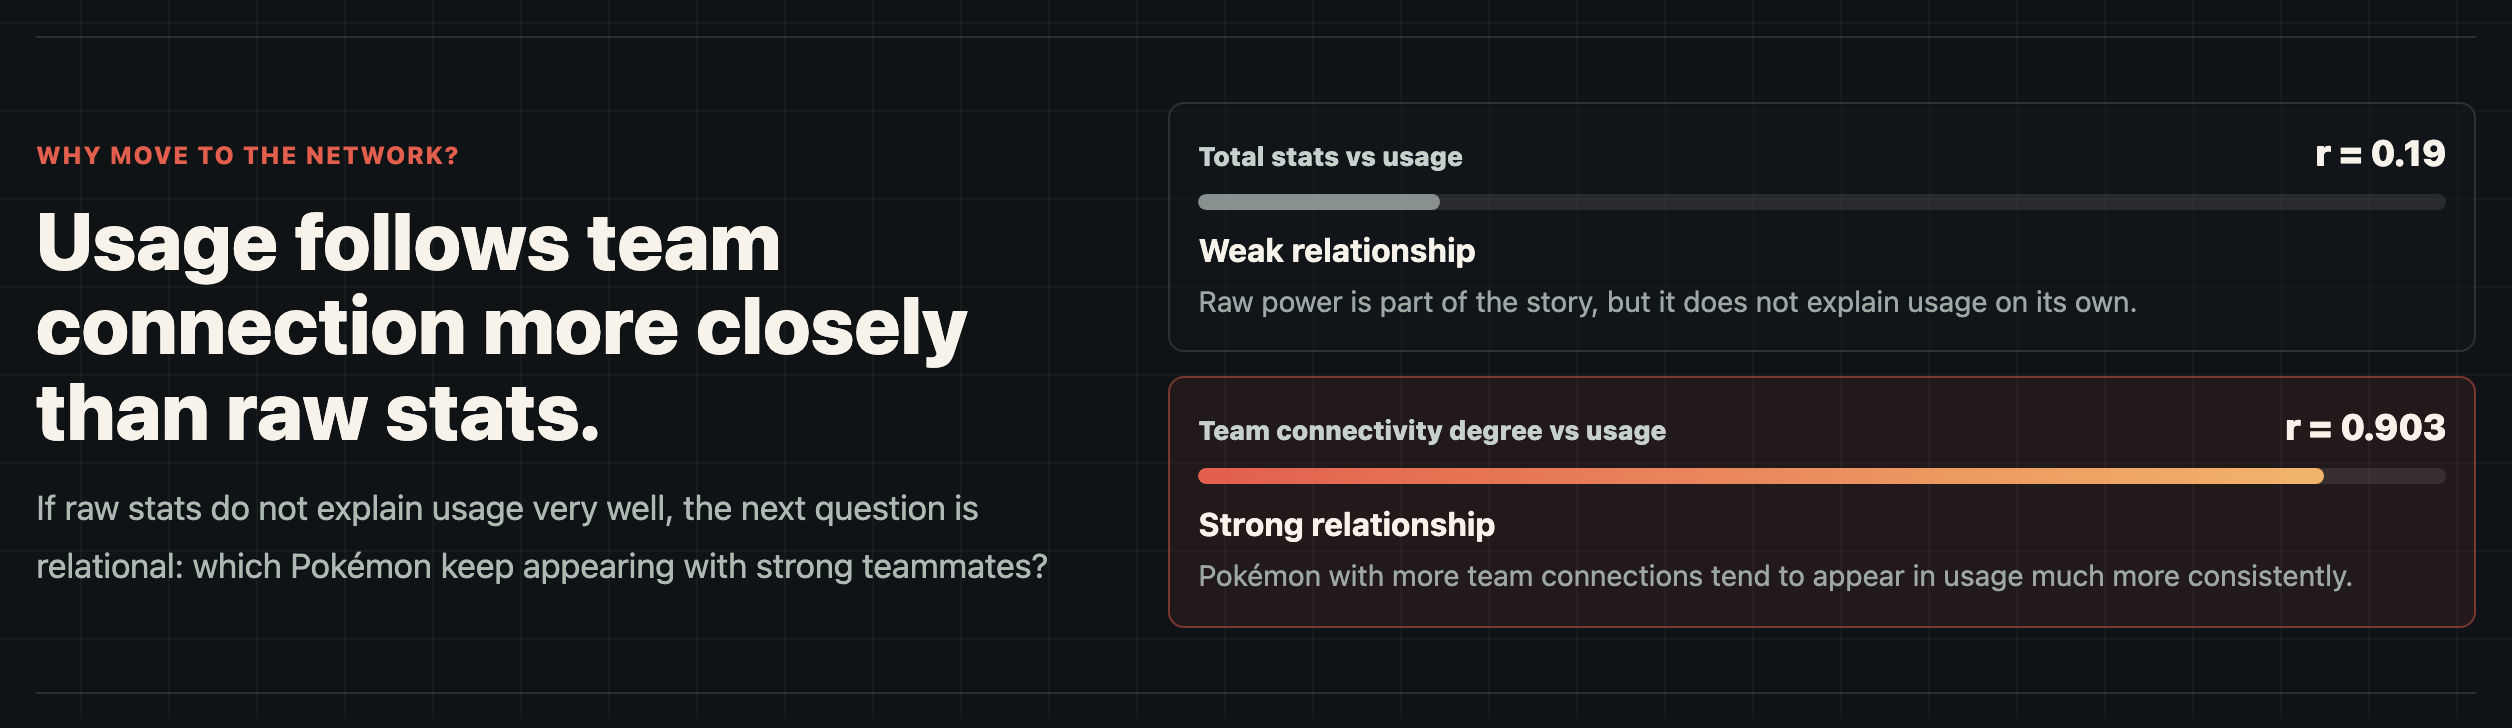
\includegraphics[width=0.84\linewidth]{figure_connectivity_bridge.png}
\smallcaption{Figure 2. The signal scan reframes the story: total stats are a weak usage signal, while connectivity degree is the strongest relationship shown in the app.}
\end{figure}

The visual encodings are intentionally consistent. In the scatterplot, x-position is base stat total and y-position is usage percentage. Color represents primary type, a red outline marks the selected Pokemon, and dashed guides make the selected point easier to read. In the network, larger nodes mean higher usage, node color again means primary type, and thicker edges mean stronger teammate co-usage. This lets users transfer what they learn from one view to another.

The key methodological move is to combine individual and relational measures. Raw base stats describe a Pokemon in isolation. Usage percentage describes metagame demand. Network degree and weighted teammate footprint describe how often a Pokemon appears in repeated team structures. Build rows for abilities, moves, and items explain why a role works. For example, Incineroar's value is not just its 530 base stat total; the detail panel highlights Intimidate, Fake Out, Parting Shot, and strong teammate links as support evidence.

\tightsection{Implementation Considerations}
The implementation is a Vite React app with D3 for charts and network layout. Data loading happens through CSV parsers in \texttt{src/App.jsx}. The app normalizes numeric values, loads image paths, computes network metrics, and builds a reduced network subset from the full teammate edge list. React state stores the selected Pokemon, comparison Pokemon, brushed scatterplot names, and active narrative step.

The most important implementation decision was shared selection. The scatterplot, network, ego-network comparison, Pokemon picker, and detail panel all respond to the same selected Pokemon. Brushing in the scatterplot clears direct selection and highlights matching network nodes. Clicking a network node or picker result updates the detail panel and comparison context. This made the page feel like one coordinated explanation rather than a collection of independent graphics.

We used supplemental image assets for Pokemon identity because small sprites make the story easier to scan. The app uses local image paths for the most important case studies and falls back to the processed image lookup table for other Pokemon. The report figures are screenshots/crops from the implemented page and are stored under \texttt{report/assets}. They document the actual interface rather than mockups.

\begin{figure}[h]
\centering
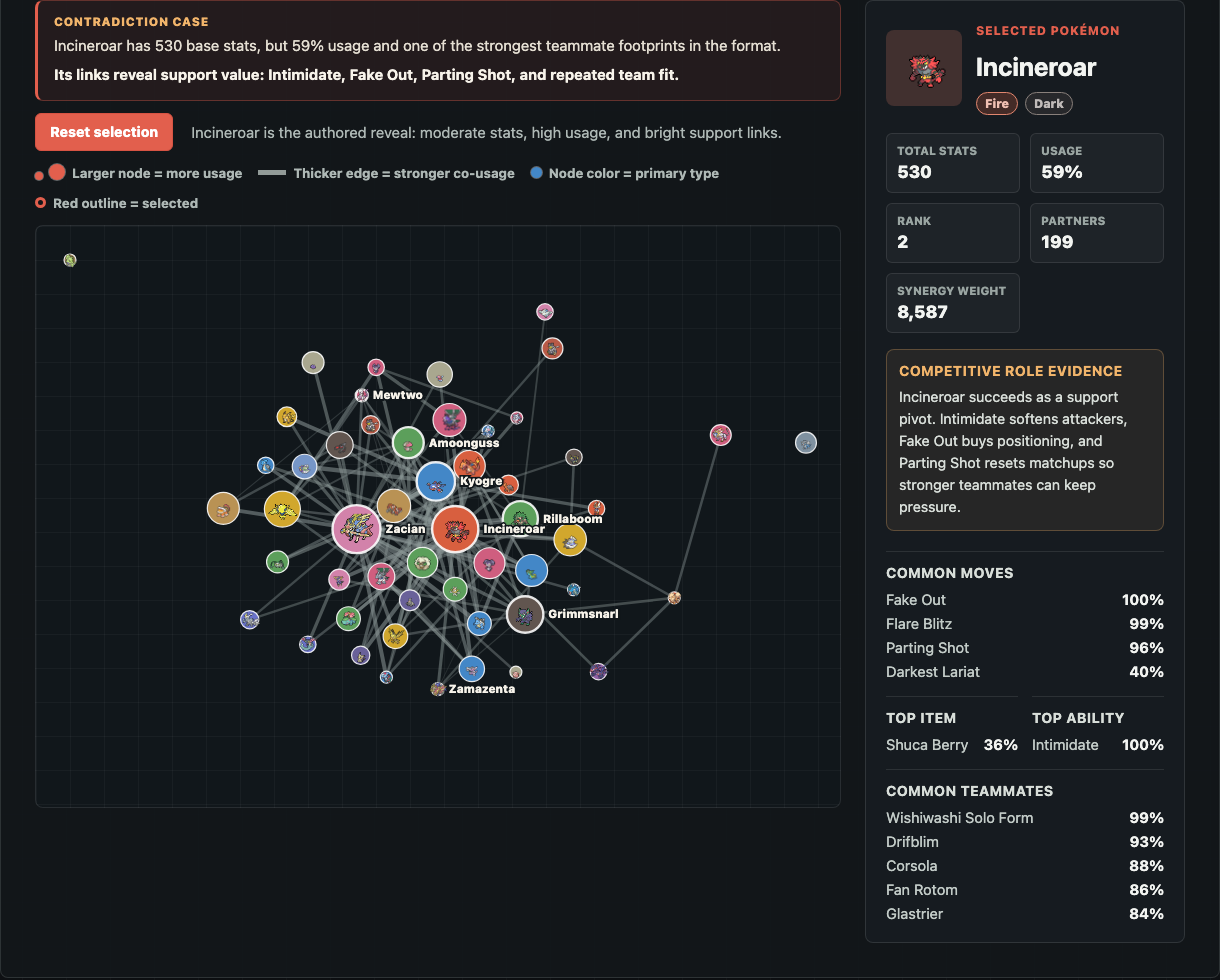
\includegraphics[width=0.92\linewidth]{figure_incineroar_network.png}
\smallcaption{Figure 3. The network reveal for Incineroar. Usage, teammate links, ego comparison, and build evidence work together to explain support value.}
\end{figure}

\tightsection{Evaluation Methods, Case Studies, and Insights}
We evaluated the project through case-study reasoning and task-based design checks. The main task was whether a viewer could explain why raw stats alone are insufficient after moving through the page. We checked whether the viewer could identify the contradiction in the scatterplot, interpret the signal scan, read network encodings, and use the detail panel to explain a selected Pokemon's role.

The most important quantitative insight is the gap between raw stats and connectivity. In the cleaned usage-tracked data, the app reports a weak total-stat/usage relationship of about \(r=0.19\), while connectivity degree is shown as a much stronger relationship with usage, about \(r=0.90\). This does not mean connectivity causes success by itself, but it strongly supports the story direction: team relationships explain competitive relevance better than base stat total alone.

The Incineroar case study is the strongest narrative example. Incineroar has only a 530 base stat total, but it has 59\% usage and one of the largest teammate footprints in the app. Its common build signals also support the explanation: Intimidate reduces pressure, Fake Out buys turns, Parting Shot supports repositioning, and repeated partners such as Zacian and Amoonguss show how it fits into team cores. Zacian Crowned Sword is a useful comparison because high stats and high usage align there. Zamazenta Crowned Shield and Mewtwo are useful counterexamples because high raw stats do not automatically produce high usage.

Qualitatively, the coordinated design improved clarity. Early versions of the project felt too much like a broad analytics dashboard. The final version works better because each section answers a specific question: What is the assumption? Where does it fail? What explains the gap? How can the reader test the pattern? The remaining limitation is that the report and app still rely on usage and co-usage rather than battle outcomes, so the claims are about observed metagame demand and team structure.

\tightsection{Directions for Further Work}
With more time, we would add win-rate or tournament-result data so that usage could be compared against direct performance. We would also improve temporal analysis by showing how usage and team cores change across months. Another useful extension would be a stronger team-builder mode: a user could select one Pokemon and see which teammates, moves, and roles form a coherent strategy.

We would also continue refining network readability. The current graph is effective for the story, but larger datasets would need clustering, filtering, and better label placement. Finally, we would run a more formal user study with novice and experienced Pokemon players to compare how each group interprets stats, roles, and team synergy.

\tightsection{Team Effort Division}
All team members have contributed a similar amount of effort. Work was shared across data cleaning, preprocessing scripts, React/D3 implementation, interface design, report writing, and presentation preparation. If the final submission requires a more detailed breakdown, we would list individual tasks, but the effort distribution for this project was broadly even.

\tightsection{References}
\vspace{-0.75em}
\renewcommand{\refname}{}
\bibliographystyle{plain}
\bibliography{references}

\end{document}
